\subsection{Governance}\label{sec:governance}

Polkadot uses sophisticated mechanisms for Governance which allows it to evolve gracefully over time at the ultimate behest of its assembled stakeholders. A key and unfailing rule is that all changes to the protocol must be agreed upon by stake-weighted referendum -- the majority of stake always commands the network.

In order to make any changes to the network, the idea is to bring dot holders and administrate a network upgrade decision with the help of the Council (Section \ref{s:council}). No matter whether the proposal is submitted by a dot holder or by the Council, it will ultimately have to go through a referendum to let all dot holders, weighted by stake, make the decision.

Each dot holder in Polkadot has the right to: a) submit a proposal, b) endorse a public proposal to prioritise it in the referendum timetable, c) vote on all active referenda, d) become a candidate for a seat in the Council, and e) vote on candidates for the Council. In addition, any dot holder may become a nominator or a validator candidate to participate in NPoS (see Section \ref{sec:validators}).

\subsubsection{Proposals and Referenda}

The core of the Polkadot logic is stored on-chain in an amorphous state-transition function and defined in a platform-neutral language: WebAssembly. Each \textbf{proposal} takes the form of a privileged function call in the runtime, that is able to modify the runtime code itself, achieving what would otherwise require a "hard fork". A proposal is then tabled and voted upon via referendum. 

Proposals can be started in one of several ways:
\begin{itemize}
\item a public proposal, which is submitted by any dot holder;
\item a Council proposal, submitted by the Council;
\item a proposal submitted automatically as part of the enactment of a prior referendum, and
\item an emergency proposal submitted by the Technical Committee (Section~\ref{s:council}).
\end{itemize} 

Each proposal approved by referendum has an associated enactment delay, i.e.~a time interval between the referendum ending and the changes being enacted. For the first two types of proposals above this is a fixed interval, tentatively set to 28 days. For the third type, it can be set as desired. Emergency proposals deal with major problems with the network which need to be fast-tracked, and hence will have a shorter enactment delay. Having an enactment delay ensures a level of stability, as it gives all parties sufficient notice to adapt to the new changes. After this period, the call to the associated privileged function is automatically made.  

Any stakeholder can submit a \emph{public proposal} by depositing a fixed minimum amount of dots, which stays locked for a certain period. If someone agrees with the proposal, they may deposit the same amount of tokens to endorse it. Public proposals are stored in a priority queue, and at regular intervals the proposal with the most endorsements gets tabled for a referendum. The locked tokens are released once the proposal is tabled.

\emph{Council proposals} are submitted by the Council, and are stored in a separate priority queue where the priorities are set at the Council's discretion.

\alfonso{}{What happens with proposals automatically submitted by the enactment of a previous referendum -- do they go to the public-proposal queue or the Council-proposal queue, or a different queue? I don't know, we should ask Gavin.}

A \textbf{referendum} is a simple, inclusive, staked-weighted voting scheme. It has a fixed voting period, after which votes are tallied. Referenda are always binary: voting options are "aye", "nay", or abstaining entirely.

\paragraph{Timetables:} Every thirty days, a new proposal will be tabled and a referendum will come up for a vote. The proposal to be tabled is the top proposal from either the public-proposal queue or the Council-proposal queue, alternating between the two queues if both are non-empty. If both queues are empty, the slot is skipped in the referendum timetable. Multiple referenda cannot be active simultaneously, except for emergency referenda which follow a parallel timetable.

\paragraph{Vote counting:} Voting on referenda is open to all dot holders with a voting power proportional to their stake, up to a possible vote multiplier which is awarded to some parties depending on their level of commitment to the system, as we explain now. A party must generally lock their tokens used for voting until at least the enactment delay period beyond the end of the referendum. This is in order to ensure that some minimal economic buy-in to the result is needed and to dissuade vote selling. It is possible to vote without locking at all, but in that case the voting power is a small fraction of a normal vote for the given stake. Conversely, Polkadot will offer \emph{voluntary extended locking}, that allows any party to increase their voting power by extending the period of time they are willing to lock up their tokens. This ensures that voters committed to the system long term, who are willing to increase their exposure to the decision of a referendum, have a greater say in the matter. In particular parachains, who lock dots when they join the network (Section~\ref{s:pAllocation}), as well as validators and nominators, who lock their stake to participate in NPoS (Section~\ref{sec:validators}), automatically benefit from a vote multiplier when they vote with their locked tokens.

\paragraph{Turnout biasing:} It may seem restrictive to force a full stakeholder-based process to do something as little as, say, nudging the block time down by $5\%$. However, without this rule the network would likely be unstable, as placing its control outside of the hands of stakeholders would create a misalignment that may lead to inaction or worse. However, by taking advantage of the fact that turnout is rarely $100\%$, we can effect different outcomes depending on the circumstances, crafting a balance of power between active and passive stakeholders. For example, simple voting systems typically introduce a notion of quorum, whereby a minimum amount of turnout must be reached before a change is passed. 

For public proposals, we generalise this notion into a "positive turnout bias", where additional turnout always makes change more likely, assuming the same yay-to-nay ratio. More specifically, in case of low turnout we favour the nay side, or status quo, by requiring a super-majority approval, and as turnout approaches $100\%$ the requirement dials down to majority-carries. This works on two principles: Firstly that the status quo tends to be safer than any change, and thus should have some bias towards it. Secondly that, like all means of empirical measurement, there is inevitably going to be some degree of inaccuracy and volatility over time, particularly when turnout is low -- a result could be $51\%-49\%$ one month and then change to $49\%-51\%$, and given the costs involved in enacting the changes of a proposal it is advantageous to ensure that a result would not likely flip shortly after enactment. 

On the other hand, for proposals submitted by the Council, referenda have no turnout bias and majority-carries is observed. The reasoning here is that proposals pre-approved by the Council are deemed safer and less likely to be reverted, so the previously mentioned issues are alleviated and we can let dot holders freely decide on the matter. 

\begin{figure}[htb]
  \centering
  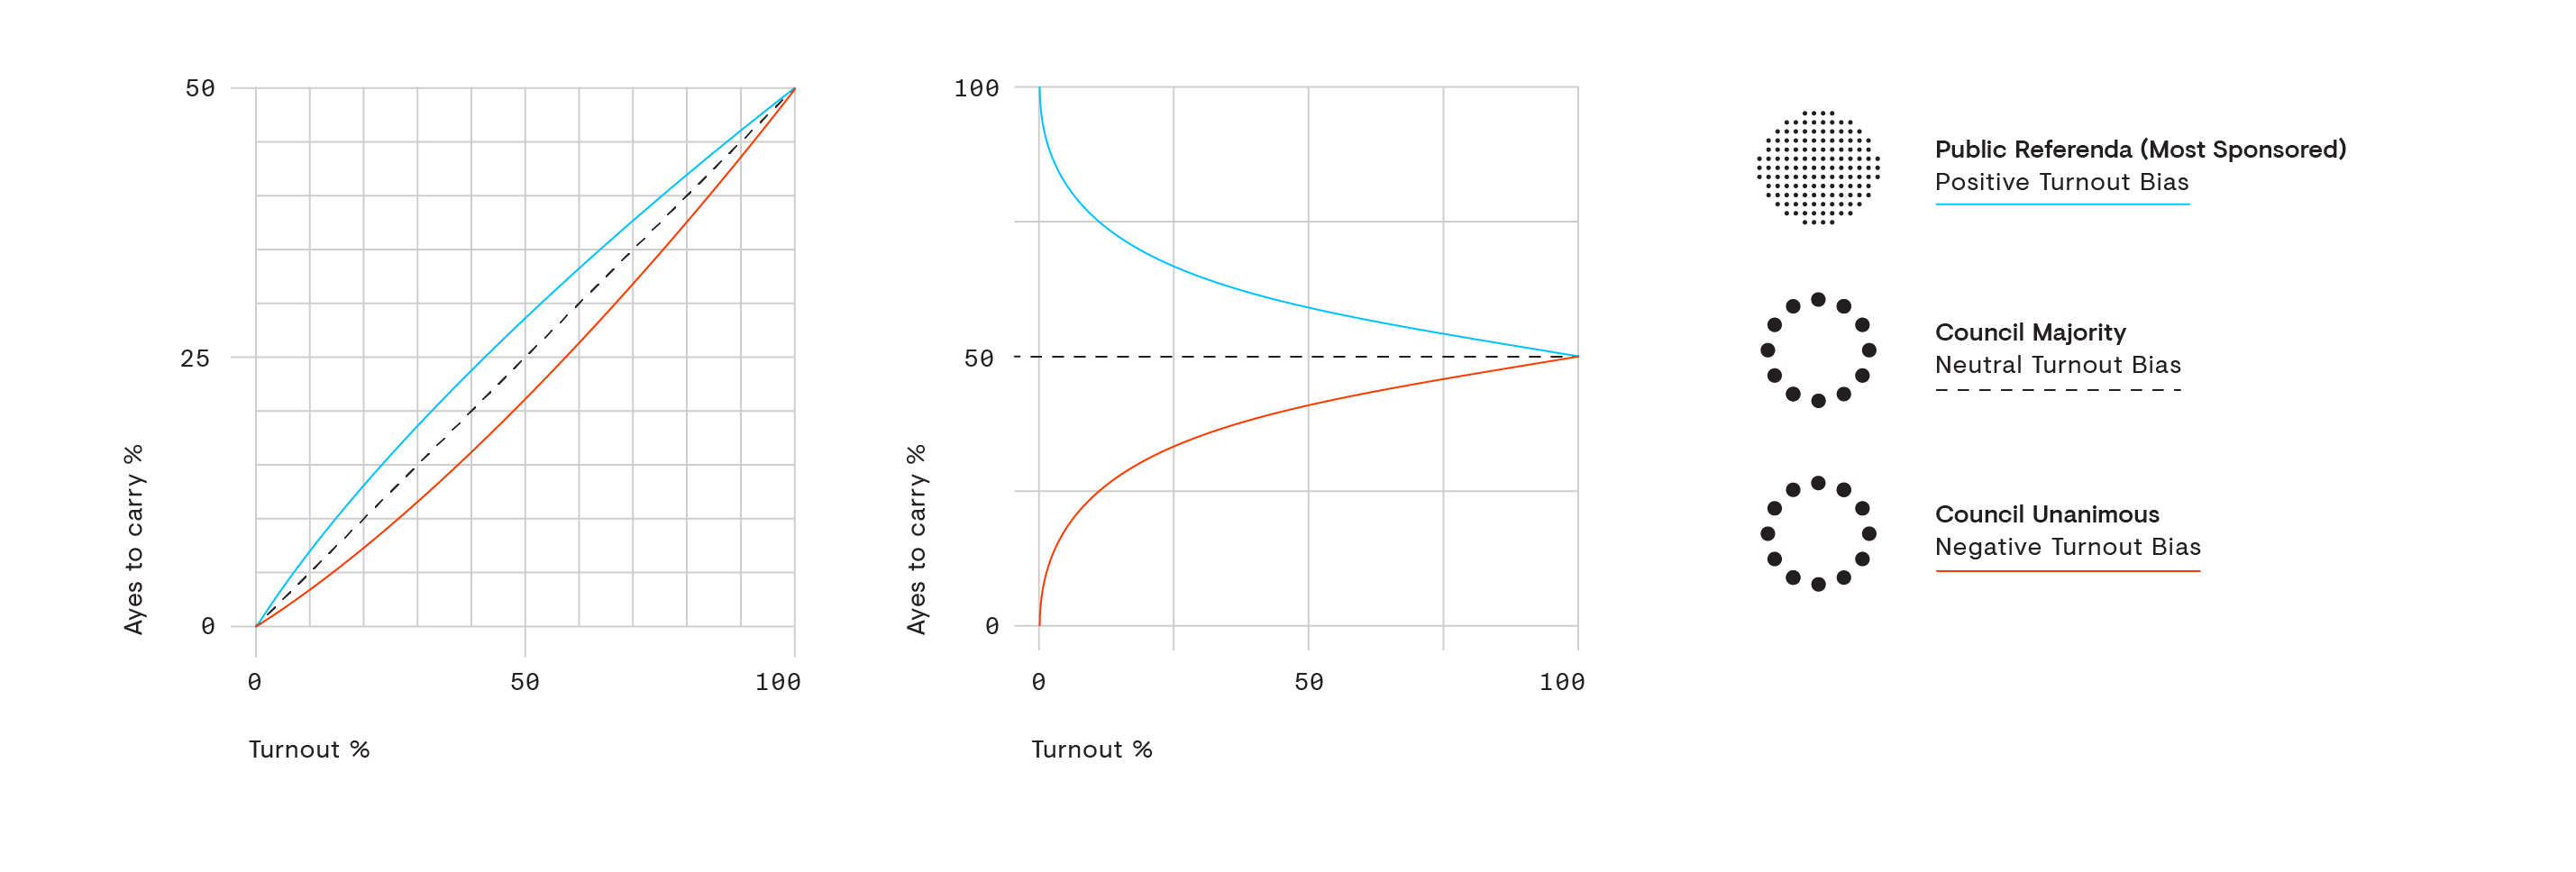
\includegraphics[width=1.1\textwidth]{images/Turnout-Bias.png}
  \caption{Adaptive turnout biasing}
    \label{fig:biasing}
\end{figure}

\alfonso{}{Alfonso: Bill proposes that the biasing should be less severe. In particular for turnout values close to zero (which is what we observe in real life) the required percentage of ayes to carry stay, say, within 33 to 66\%, instead of going all the way to 0 or 100\%. I agree with him.}

Finally, in the exceptional case that a Council proposal receives unanimous support by all Council members, it will observe a "negative turnout bias". This is the symmetric opposite of the first case, where additional turnout always makes change less likely, we favour the yay side in case of low turnout by requiring a super-majority of nays to reject the proposal, and as turnout approaches $100\%$ the requirement dials down to majority-carries. See Figure~\ref{fig:biasing}.


\subsubsection{The Council and the Technical Committee}\label{s:council}

\textbf{The Council} is an entity comprising a number of actors each represented by an on-chain account. Its goals are to represent passive stakeholders, submit sensible and important proposals, and cancel uncontroversially dangerous or malicious proposals.

The Council will constantly review candidate proposals to deal with emerging issues in the system. A candidate proposal is officially backed by the Council -- and enters the queue of Council proposals -- only after it is approved by a strict majority of Council members, with no member exercising a veto. A candidate proposal can be vetoed only once; if, after a cool-down period, it is once more approved by a majority of Council members, it cannot be vetoed a second time. 

\alfonso{}{The Council should have the capacity to change the bias of any proposal through majority voting or unanimity, even a public proposal. Is this the case now?}

As mentioned before, in the case that all members vote in favour, a Council proposal is consider uncontroversial and enjoys a special turnout bias that makes it more likely to be approved. 

Finally, Council members may vote to cancel any proposal, regardless of who submitted it, but their vote must be unanimous. Since unanimity is a high requirement, it is expected that this measure will only be used when it is an entirely uncontroversial move. This may function as a last resort if there is an issue found late in the day with a referendum's proposal such as a bug in the code of the runtime or a vulnerability  that the proposal would institute. If the cancellation is controversial enough that there is at least one dissenter, then it will be left to all dot holders en masse to determine the fate of the proposal, with the registered Council cancellation votes serving as red flags so that voters pay special attention.

\paragraph{Electing Council members:} At Polkadot Genesis, there will be 6 to 12 seats in the Council, and an extra seat will be added every two weeks, ultimately settling at 24 seats.  All Council members have a fixed term of one year, and a member can be removed early only by referendum. 

All dot holders are free to register their candidacy for the Council, and free to vote for any number of candidates, with a voting power proportional to their stake. A general election for the 24 Council seats will take place once a year. Much like the validator election problem in NPoS, this is a stake-weighted, multi-winner election problem based on approval ballots. We can thus solve it using the same algorithm we use for NPoS, which in particular offers the property of \emph{proportional justified representation}; see Section~\ref{sec:validators} for more details. This property guarantees that the elected Council will represent as many minorities as possible, thus ensuring that Governance stay decentralised and resistant to capture. Council members can be re-elected indefinitely, provided their approval remains high enough. 

\medskip

\textbf{The Technical Committee} is composed according to a single vote for each team that has successfully and independently implemented or formally specified the protocol in Polkadot, or in its canary network Kusama\footnote{http://kusama.network}. Teams may be added or removed by a simple majority of the Council. 

The Technical Committee is the last line of defence for the system. Its sole purpose is detecting present or imminent issues in the system such as bugs in the code or security vulnerabilities, and proposing and fast-tracking emergency referenda. An emergency proposal needs a simultaneous approval of at least three-quarters of the Council members and at least two-thirds of the Technical Committee members in order to be tabled. Once tabled, it is fast-tracked into a referendum that runs in parallel with the timetable of regular referenda, with a far shorter voting period, and a near-zero enactment period. The approval mechanics in this case are unchanged from what they would be otherwise, i.e.~either a simple majority or, in the case of a unanimous Council approval, a turnout-based bias for approval.

We highlight that for practical reasons the Technical Committee is not democratically elected, but in contrast it has an extremely reduced scope of action and no power to act unilaterally, as explained in the lines above. This mechanism is expected to suffice for non-contentious bug fixes and technical upgrades, but given the requirements imposed, may not be effective in the case of emergencies that have a tinge of political sensitivity or strategic importance to them. 
 
\subsubsection{Allocation of parachain slots}\label{s:pAllocation}

We use auctions to have a fair, transparent and permissionless parachain allocation procedure. 
Broadly speaking, parties interested in receiving a parachain slot participate in an auction with dot-denominated bids. The party with the highest bid is declared as winner and is allocated a slot for a specific period of time, with its bid becoming a locked deposit that is released at the end of said period. The leasing cost of the slot thus corresponds to the opportunity cost of having this deposit locked. This dot-denominated deposit also establishes the voting power of the parachain in Polkadot's governance.

Since implementing seal-bid auctions is difficult and in order to avoid bid sniping, we adopt a Candle auction \cite{Fuellbrunn:2012:CandleAuction} mechanism with a retroactively determined close. 
Going into detail, we plan to have an auction every few weeks, where in each auction four contiguous six-month slots are offered for lease. A bid can be made for any combination of one, two, three or four contiguous slots, for a total of ten possible time periods lasting 6, 12, 18 or 24 months. Once the auction starts, parties can post bids as transactions for any one of these ten periods, within a fixed window of time lasting several hours. A party is allowed to submit multiple bids, where a bid is registered only if a) it beats the current highest bid for the corresponding period, and b) the party does not become the provisional winner of two or more periods with gaps in between. For example, the winner of period $(1,2)$ -- constituted of the first two slots -- cannot bid on period $(4)$ -- the fourth slot -- until someone else overbids the former period. 

%A special data structure which allows us to 
We keep track of the provisional winners of all 10 periods at each point in time throughout the bidding time-window. Once this window is over, a public random number retroactively establishes a closing time within this window, thus also establishing a winner for each period.%
\footnote{More precisely, one of the blocks produced during the bidding time-window is selected by a public pseudo-random function, and all bids processes after that block are ignored. A cryptographic guarantee ensures that the pseudo-random function cannot be biased by any minority controlling less than 1/3 of the block production, with overwhelming probability.} %
The final winners correspond to the subset of non-overlapping periods with highest average bid per slot. For example, let us assume that at closing time we have the following winning bids: 75 dots for period $(1,4)$, 30 dots for period $(1,2)$, 90 dots for period $(3,4)$, and 100 dots for period $(2,3)$. In this example, set $[(1,2), (3,4)]$ has an average bid per slot of $(2\times 30 + 2\times 90)/4 = 60$, set $[(1,4)]$ has an average of $(4\times 75)/4 = 75$, and set $[(2,3)]$ has an average of $(0+2\times 100+0)/4=50$, so the final winner is set $[(1,4)]$. 

The stated goals of this design are to incentivise parties to bid early and avoid bid sniping, to give less funded projects a chance of winning a slot hence securing the decentralised nature of Polkadot, and to discourage grieving attacks by parties who raise the value of the winning bid with no intention of winning themselves.

\subsubsection{Treasury}\label{sec:treasury}

 The system needs to continually raise funds which we call the Treasury.
 These funds are used to pay for developers that provide software updates, apply any changes decided by referenda, adjust parameters, and generally keep the system running smoothly. Funds may also be used for further goals such as marketing activities, community events and outreach. This is ultimately controlled by all dot holders via Governance and it will be the community and their collective imagination and judgment which really determines the course of the Treasury.

Funds for Treasury are raised in two ways:

\begin{enumerate}
\item by minting new tokens, leading to inflation, and
\item by channeling a fraction of transaction fees and of slashings.
\end{enumerate}

 
Notice that these methods to raise funds mimic the traditional ways that governments raise funds: by minting coins which leads to controlled inflation, and by collecting taxes and fines.
We could raise funds solely from minting new tokens, but we argue that it makes sense to redirect into Treasury some of the tokens from transaction fees and slashing that would otherwise be burned. By doing so, we reduce the amount of actual stake burning, and this gives us better control over the inflation rate, since stake burning leads to deflation and we cannot control the events that lead to burning. Furthermore, following an event that produced heavy stake slashing, the system is likely to need additional funds to develop software updates or new infrastructure that deal with an existing issue, or it might be decided by Governance to reimburse some of the slashed stake. Thus, it makes sense to have the slashed dots available in Treasury, instead of burning them and having to mint more dots soon thereafter.
